
\chapter{Neurónové siete}\label{chap:neuralnet}

Keďže \textit{umelé neurónové siete} sú významnou časťou tejto práce, venujeme im samostatnú kapitolu. Popíšeme čo sú neurónové siete, ako fungujú a základné typy neurónových sietí, ktoré používame v aplikácií.
\bigskip

\section{Jednoduchý spojitý perceprtón}

\begin{figure}[hp]
  \begin{center}
    \begin{subfigure}[b]{0.6\textwidth}
      \centering
      \includegraphics[width=\textwidth]{images/bio_neuron}
      \caption{Prírodný neurón}
      \label{fig:bio_neuron}
    \end{subfigure}
    \begin{subfigure}[b]{0.3\textwidth}
      \centering
 	  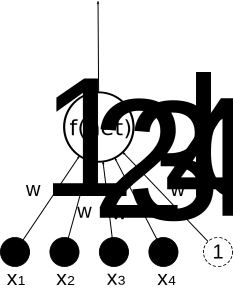
\includegraphics[width=\textwidth]{images/neuron}
 	  \caption{Umelý neurón}
 	    \label{fig:neuron}
    \end{subfigure}
  \end{center}%  
  \caption{Prírodný vs. umelý neurón}
\end{figure}

Jednoduchý perceptrón je inšpirovaný nervovou bunkou - neurónom. Vstupy umelého neurónu zodpovedajú \textit{dendridom}, výstup zodpovedá \textit{axónu}. 
Transformáciu vstupu na výstup zabezpečuje aktivačná funkcia.

Keď si neurón predstavíme ako orientovaný graf, za vrcholy položíme, vstupy, výstup a ,,telo" neurónu, vzniknú nám 2 typy hrán.
\begin{enumerate}
\item Synaptické -- vstup $\rightarrow$ neurón -- lineárna input-output väzba, kde pôvodný signál $x_i$ prenásobíme váhou synapsy $w_i$ a tým dostaneme výsledný signál $x_i'$.

\item Aktivačné -- neurón $\rightarrow$ výstup -- nelineárna input-output väzba, kde $y$ dostaneme dosadením $\sum x_i'$ do aktivačnej funkcie.
\end{enumerate}

K vstupom treba pridať ešte jeden vstup -- \textit{bias} -- ktorý má vždy hodnotu 1. Jeho význam je pri vstupe so samými nulami, pretože vtedy hodnoty na synapsách ostanú nezmenené a perceptrón by sa tento vzor nevedel naučiť.

Nech $n$ je počet vstupov a  $f$ je aktivačná funkcia. Výsledný signál $y$ dostaneme takto:
$$y= f\left(\sum_{i=1}^{n+1} w_i x_i \right)\qquad x_{n+1}=1$$

Aktivačnou funkciou spojitého je sigmoida: 
$$f(x) = \frac{1}{1+e^{-x}}$$
Sigmoida bola vybratá preto, lebo spĺňa vlastnosti, ktoré má mať aktivačná funkcia.

Takýto perceptrón robí zobrazenie $\mathbb{R}^n\rightarrow (0,1)$.

%\section{Vrstva neurónovej siete}

%\textbf{Vrstva neurónovej siete} sa skladá z niekoľkých jednoduchých spojitých perceptrónov (neurónov). Každý neurón sa aktivuje samostatne - nezávisle od ostatných.

%Vrstva robí zobrazenie $\mathbb{R}^n\rightarrow (0,1)^m$, kde $n$ je rozmer vstupu a $m$ je počet neurónov vo vrstve.
